
%%%%%%%%%%%%%%%%%%%%%%%%%%%%%%%%
%------------------------------%
%%%%%%%%%%%%%%%%%%%%%%%%%%%%%%%%
\section{Introduction}
%%%%%%%%%%%%%%%%%%%%%%%%%%%%%%%%
%------------------------------%
%%%%%%%%%%%%%%%%%%%%%%%%%%%%%%%%

An objective of many genetic studies is to accurately identify variants associated with a particular trait or disease, and to estimate the effects of those variants. Such information is valuable for assessing an individual's risk of developing a particular condition, elucidating the underlying genetic architecture of a disease, and identifying potential drug targets. However, this effort may be hindered by several factors. 

Genetic variants are often correlated with each other, meaning that univariate testing of genetic variants may result in false positives and biased effect estimates. This occurs when the variant being tested is correlated with other variants, so that the effects of these correlated variants are erroneously attributed to the variant in question. One method for analyzing data in the presence of LD is pruning, where only uncorrelated SNPs are used in modeling or testing procedures. Pruning limits analysis to SNPs which are representative of a particular region, and may result in improved predictive accuracy. However, pruning is limited in that it can only identify SNPs in LD with the true causal SNP. In addition, it has been shown that a worst-case scenario, pruning algorithms may not select any representative SNPs in a particular region of the genome \cite{prive2018efficient}.

An alternative solution to the problem of LD is the use of multivariate methods such as multiple linear regression, which adjusts for and estimates the effects of numerous variants simultaneously. However, such methods rely on data where the number of observations is less than the number of of features. This is often infeasible in genetic studies where the number of features frequently exceeds the number of observations. Penalized regression methods make such problems tractable, by constraining the solution space of coefficient estimates.

The Lasso \cite{tibshirani1996regression} is a widely used penalized regression method. It relies on an assumption of sparsity, which allows for computational speedup while performing coefficient estimation and variable selection simultaneously. These features make the Lasso attractive for the analysis of high-dimensional genetic data where identifying a list of variants most highly associated with a particular trait is often of interest.

Lasso penalized regression models assume independent observations and uncorrelated errors. In the presence of population structure, some samples are more correlated than others, violating the independent errors assumption. If left unaccounted for, this presence of such dependency can result in the identification of spurious associations. Though methods to correct for population stratification and cryptic relatedness have been extensively investigated \cite{Amin2007, hoffman2013correcting, price2006principal, Rakitsch2012, bhatnagar2019simultaneous, Sillanpaeae2011}, there remain open and relevant problems in analyzing structured genetic data \cite{lawson2019population, barton2019population}. 

One reason that population stratification warrants such concern in genetic studies is that due to ethnic and geographic segregation, population stratification tends to be associated with differing environmental exposures and cultural practices.  In other words, random genetic variation is likely to be associated with non-genetic factors that also influence the trait of interest, thereby confounding the genotype-phenotype relationship and leading to spurious associations and biased estimates of SNP effects. Biased estimates of this nature severely hinder prediction and understanding differences among populations \cite{barton2019population}. Although bias at individual loci may be small, this bias may become magnified when aggregated across thousands of SNPs, as is done when calculating polygenic risk scores \cite{barton2019population}.


In order to clarify and emphasize the importance of this subtle distinction, we present a detailed review of relevant concepts and methods. The remainder of this paper is organized as follows. In section \ref{structureSources} we provide a summary of the causes and consequences of structure in the genetic data of seemingly unrelated individuals and formally define terminology used throughout this paper. We emphasize that confounding due to population structure, frequently cited as a driver of spurious associations \cite{Sillanpaeae2011, sul2018population} \anna{other papers? NB: re-read Sul, 2018 paper - a lot of similar review concepts}, is a function of environmental heterogeneity, where genetic data serves as a proxy for differential environmental exposures. In so doing, we refine the definition of confounding due to population structure in terms of a non-genetic mechanism. In section \ref{methodsHistorical} we briefly review historical methods of correcting for population stratification and relatedness. In section \ref{methodsFixedRandom} we review methods of correcting for population stratification as a fixed versus random effect. These correspond to PCA adjusted lasso penalized regression and lasso penalized multivariate LMMs, respectively, the two most prevalent multivariate methods of adjusting for population stratification and relatedness at present. In addition, we review the statistical details of the consequences of population structure and heterogeneous environmental exposures for these methods. In sections \ref{simulation} and \ref{results}, we illustrate the concepts described in section \ref{methodsFixedRandom} via simulation studies, where the data-generating mechanism formally differentiates between population structure and environmental heterogeneity. These simulation results are used to illustrate the importance of distinguishing between population structure and heterogeneous environmental exposures in penalized LMMs.





%%%%%%%%%%%%%%%%%%%%%%%%%%%%%%%%
%------------------------------%
%%%%%%%%%%%%%%%%%%%%%%%%%%%%%%%%
\section{Background}
%%%%%%%%%%%%%%%%%%%%%%%%%%%%%%%%
%------------------------------%
%%%%%%%%%%%%%%%%%%%%%%%%%%%%%%%%

%------------------------------%
\subsection{Structure in genetic data}

Population structure is a common phenomenon in genetic data. Varying levels of relatedness are almost always present among genetic samples, even in samples of unrelated individuals and seemingly homogeneous populations. For example, European American \cite{campbell2005demonstrating}, Han Chinese \cite{xu2009genomic, chen2009genetic}, and most recently, cohorts within the UK Biobank data \cite{haworth2019apparent}.

Relatedness describes how genetically similar individuals are, and can refer to both ancient and recent relatedness.  Recent relatedness is characterized by small clusters of high levels of similarity and is indicative of familial or cryptic relatedness. Ancient relatedness, or common ancestry, is generally characterized by large clusters of low levels of similarity. The presence of multiple distinct ancestry groups is known as population stratification. 

Pedigree-based methods may be used to explicitly model recent relatedness if familial relationships are known. However, in this review we focus on methods to account for unobserved relatedness. Throughout this paper, the terms \textbf{population structure} and \textbf{structured population} will be used to describe a sample of individuals in which population stratification, cryptic relatedness, or both are be present. Population stratification in particular has been of great concern in genetic studies due to its potential to lead to spurious associations. This phenomenon is commonly described as \textbf{confounding due to population stratification}. However, the mechanism of this phenomenon warrants some discussion. In particular, it is often overlooked that population structure itself does not confound the genotype-phenotype relationship in the classical sense, rather there must exist some non-genetic mechanism by which population stratification affects both the phenotype and genotype \cite{barton2019population, vilhjalmsson2012nature}. \\

\anna{DAG here with only population stratification, observed snps, and phenotype ... maybe an arrow from population stratification to phenotype with a question mark (?)}


%------------------------------%
\subsection{Motivating example}

As an example, consider a genetic study to assess genetic variants associated with lung cancer in a sample comprised of subjects from two distinct subpopulationsk A and B. Assume the major allele of SNP $X$ is present with higher frequency in subpopulation A compared to subpopulation B, but it has no direct effect on lung cancer. Now suppose these subpopulations are geographically segregated in a such a way that subpopulation A is exposed to good air quality, and subpopulation B to poor air quality. A GWAS analysis of data from these subpopulations would find SNP $X$ to be significantly associated with lung cancer. This spurious association is not identified because of the presence of population stratification itself, but because that stratification is related to a causal environmental exposure. Indeed, if subpopulations A and B were not subject to different air qualities, all else being equal, SNP $X$ would not be found to be associated with the phenotype.\\

\anna{description of DAG below, in reference to previous one}

The mechanism of environmental confounding is summarized in the directed acyclic graph displayed in figure \ref{fig:ps_env}. The undirected dashed line between population stratification and environmental exposure indicates that while we assume these elements are correlated, we do not assume any causal direction. Otherwise stated, we do not assume that environmental factors influence population-specific allele frequencies, or vice versa, only that the two may be related. Additionally, we assume that the environmental exposure has no effect on on observed SNPs.

\begin{figure}[H]
\centering
\begin{tikzpicture}[%
>=latex',
circ/.style={draw, shape=circle, node distance=1cm, line width=1pt}]%Define the arrow type and style for circled nodes
\draw[dashed] (0,1) node[left] (P) {Population Stratification} -- (2,1) node[right] (E) {Environment}; 
\draw[->] (0,0) node[left] (X) {Observed SNPs} -- (2,0) node[right] (Y) {Phenotype}; %Line between X and Y
\draw[->] (P)   -- (X) ; 
\draw[->] (E)   -- (Y) ; 
% \filldraw[color=red!60, fill=none, very thick] (0,1) ellipse (4.5 and 0.35);
\end{tikzpicture}
\end{figure}

\anna{An additional consideration in genetic studies that we briefly review  is that of genetic background. Genetic background describes when SNPs that have a causal relationship with the phenotype of interest are not directly observed, but are correlated with SNPs that are observed. As \cite{vilhjalmsson2012nature} note, any trait that has some genetic basis will be subject to genetic background effects, just as traits that are influenced by the environment may be subject to environmental confounding. Given the importance of both genetic and environmental contributions to many complex phenotypes, both genetic background and environmental confounding are important factors in our ability to identify true causal genetic relationships between SNPs and phenotype. }

\anna{
This work will focus on environmental confounding, however, we wish to acknowledge and describe genetic background as a potential confounder for the sake of completeness. 
}



%------------------------------%
\subsection{Correcting for population structure}

Statistical methods to control for the effects of confounding due to population stratification have proliferated as computational advances have allowed for the analysis of genetic data from large cohorts. It should be noted that by attempting to reduce the effects of population structure, these methods reduce the effects of environmental confounding by blocking the casual pathway between population structure and observed SNPs.

The genomic control method is a univariate testing procedure which modifies the Cochran-Armitage test for trend by a correction factor. This correction attempts to quantify and remove the effect of population structure on the distribution of the chi-square statistic using markers unrelated to the phenotype of interest and independent of the marker being tested for association \cite{devlin1999genomic, bacanu2000power, wang2009testing}. The genomic control method retains the disadvantages of univariate SNP testing and its power to detect true associations is likely to suffer in the presence of linkage disequilibrium. 

The structured association method attempts to infer subject membership within a discrete number of nonoverlapping subpopulations. Subsequent analyses are conducted within each subpopulation, and the subpopulation-specific results may then be combined via meta-analysis \cite{pritchard1999use, pritchard2000association}. By partitioning the overall sample size in this manner, the structured association method is particularly vulnerable to a loss of power. Additionally, it relies on the assumption that these subpopulations are distinct and nonoveralapping. This assumption may not accurately reflect the characteristics of a particular sample, such as one consisting of admixed populations, or recent relatedness. Considered in the context of our air quality example, rather than the existence of two subpopulations with exposure to either good or bad air quality, there may also be individuals who fall somewhere between these two extremes. By clustering those individuals within in one subpopulation or another we lose information about more high dimensional relatedness.

Another approach is to create an approximation of population structure using surrogate variables, and to adjust for these as an additional model covariates. Principal component-adjustment (PC-adjustment) methods use the first several principal components of the design matrix as these surrogate variables \cite{price2006principal}. This approach may be used in univariate or multivariate frameworks, and allows for analysis on the entirety of a structured sample. 

Like PC-adjustment methods, LMMs rely on a pair-wise similarity matrix to estimate and subsequently correct for relatedness among subjects. However, the term LMM has been used to describe a number of distinct procedures for analyzing structured genetic data which differ in their objectives and methods. There are two main objectives of LMMs used in a structured genetic context: estimating narrow-sense heritability, and estimating individual SNP effects.

Among LMM methods that aim to estimate heritability, the most well-known example is genome-wide complex trait analysis (GCTA) \cite{yang2011gcta}. In this framework, all observed SNPs are treated as random effects. These effects are integrated out in order to estimate a genetic variance component, which in turn, is used to quantify the total narrow-sense heritability of a trait \cite{yang2010common}. \anna{We will briefly return to a discussion of GCTA and related methods later, though techniques for estimating heritability are not the focus of this paper.}

Within the category of LMMs that aim to estimate SNP effects are univariate and multivariate approaches. Univariate approaches attempt to estimate univariate SNP effects on phenotype and assess the statistical significance of SNP-phenotype associations while controlling for population structure using a genetic similarity matrix \cite{yu2006unified, kang2010variance, kang2008efficient}. However, as with all univariate testing approaches univariate LMM implementations may still produce spurious associations and biased effect estimates in the presence of LD. 

Multivariate mixed model approaches reduce these problems by assessing the relationship between a phenotype of interest and all SNPs simultaneously via penalized regression, while controlling for environmental confounding  \cite{Rakitsch2012, bhatnagar2019simultaneous}. This approach assumes there are a relatively small number of SNPs associated with the phenotype of interest that have large effect sizes. These SNPs will be included in the model as both fixed and random effects, while SNPs with smaller effect sizes are modeled only as part of the random effect in order to control for environmental confounding. \\

\anna{say more about logistic?}\\
The remainder of this review will focus on the performance of multivariate Lasso-penalized methods for the analysis of continuous, normally distributed outcomes. Specifically, PC-adjustment and LMM methods, which we will refer to as PC-Lasso and LMM-Lasso, respectively. We consider two similar implementations of the LMM-Lasso method, one developed by \cite{Rakitsch2012} and a more recent implementation from \cite{bhatnagar2019simultaneous}. Subsequent references to LMM-Lasso apply to both implementations, unless otherwise stated. Where necessary, we will differentiate between these implementations as LMM-Lasso-Rakitsch and LMM-Lasso-ggmix, respectively. 

Using simulations, we compare the performance of PC-Lasso and LMM-Lasso in terms of their abilities to accurately estimate SNP effects and in terms of their true sign rates in the presence of varying levels of relatedness and environmental confounding. \\

\anna{Do we want to include the sign rate stuff?}

Although several studies have shown that LMMs outperform PC-adjustment methods in the univariate framework \cite{wang2013analytical, kang2010variance, zhao2007arabidopsis}, to the best of our knowledge this is the only comprehensive review and comparison of these methods in a penalized multivariate framework and using a simulation scheme motivated by human genetic relatedness and which formalizes the non-genetic confounding mechanism of population stratification.\\

\anna{find that 2020 paper that simulates the data sort of similarly}


%%%%%%%%%%%%%%%%%%%%%%%%%%%%%%%%
%------------------------------%
%%%%%%%%%%%%%%%%%%%%%%%%%%%%%%%%
\section{Methods}
%%%%%%%%%%%%%%%%%%%%%%%%%%%%%%%%
%------------------------------%
%%%%%%%%%%%%%%%%%%%%%%%%%%%%%%%%



%------------------------------%
\subsection{Model}

To describe and compare PC-Lasso and LMM-Lasso, we consider an $n \times p$ matrix of genotype data $\boldsymbol{G}$ for $n$ subjects belonging to $q \le p$ subpopulations and $p$ SNPs, where each $G_{i,j} \in \{ 0, 1, 2 \}$ enumerates the number of allele copies subject $i$ has for SNP $j$. We denote the standardized version of this genotype matrix as $\bX$. We assume that an $n \times 1$ vector of continuous phenotype values, $\by$, can be expressed as the sum of additive SNP effects, environmental confounding, and observational noise and consider the linear mixed model,

\begin{equation}
    \label{eqn:model}
    \by = \bX\bbeta + \bZ\bgamma + \beps
\end{equation}

where $\bbeta$ is a $p \times 1$ vector of SNP effects, $\bZ$ is an $n \times q$ matrix that indicates population structure, $\bgamma$ is an $q \times 1$ vector of subpopulation-specific environmental effects, and $\beps \sim N(\boldsymbol{0}, \sigmaee \bI_n)$.

Both PC-Lasso and LMM-Lasso rely on matrix decompositions of $\bX$ and relative relationship matrix (RRM), $\bK$, which describes the pair-wise genetic similarity among subjects \cite{hayes2009increased}. Using the singular value decomposition (SVD) of the standardized genotype matrix, we can derive the spectral decomposition of the RRM:

\begin{align}
    \label{eqn:k}
    \bK &= \frac{1}{p} \bX \bX^T \nonumber \\
                   &= \frac{1}{p} \bU \bD^2 \bU^T \nonumber \\
                   &= \frac{1}{p} \bU \bD (\bU \bD)^T \nonumber \\
                   &\propto \bR \bR^T
\end{align}

where the columns of $\bU$ are the principal components of $\bX$ (equivalently, those of $\bK$) and $\boldsymbol{D}^2$ is a diagonal matrix of the eigenvalues of $\bX$ (equivalently, the singular values of $\bK$.) The columns of $\boldsymbol{R}$ are therefore proportional to the principal components weighted by their corresponding singular values. 

%------------------------------%
\subsection{PC-Lasso}
PC-Lasso uses the first $k$ principal components of $\bX$ to approximate $\bZ\bgamma$ and includes them in the model as unpenalized covariates. It has been shown \cite{hoffman2013correcting} that this corresponds to the regression model

\begin{equation}
    \label{eqn:pca_reg}
    \by = \bX\bbeta + \bU_{1:k}\boldsymbol{\alpha} + \beps 
\end{equation}

where $\bU_{1:k}$ is the $n \times k$ matrix of principal component vectors, $\boldsymbol{\alpha}$ their corresponding $k \times 1$ coefficient vector, and all other parameters are as defined in equation \ref{eqn:model}. In a penalized regression framework, this model yields the objective function

\begin{equation}
    \label{eqn:pca_obj}
    Q(\boldsymbol{\beta, \alpha| X, y}) = \frac{1}{2n} ||\boldsymbol{y} - \boldsymbol{X \beta} - \bU_{1:k}\boldsymbol{\alpha}||_2^2 + \lambda || \boldsymbol{\beta} ||_1
\end{equation}

where $\lambda$ is a tuning parameter, and $|| \boldsymbol{\beta} ||_1 = \sum_{j=1}^p |\beta_j|$ denotes the $\ell_1$ norm of the regression coefficients. \anna{do I need to define the ell2 norm?} Note that the principal component regression coefficients, $\boldsymbol{\alpha}$, are not included in the penalty term. 

%which requires estimation of $p + k + 1$ parameters. Determining the appropriate number of principal components to include is a non-trivial task. However, often in practice the first 10 principal components are used. \anna{and so that's what we do in all our analyses.} 



%------------------------------%
\subsection{LMM-Lasso}
LMM-Lasso models $\bZ\bgamma$ as a random effect assuming $\bgamma \sim N(\boldsymbol{0}, \sigmagg / p \bI_p)$. Often $\bZ$ is not observed directly, and a common convention is to replace $\bZ$ with $\bX$, yielding the random effect $\bX\bgamma \sim N(\boldsymbol{0}, \sigmagg \textbf{K})$. \anna{Equivalently, $\bX\bgamma$ may be denoted $\boldsymbol{u} \sim N(\boldsymbol{0}, \sigmagg \bK)$.} This results in the following LMM regression model

\begin{equation}
    \label{eqn:lmm_reg}
    \by = \bX\bbeta + \bX\bgamma+ \beps
\end{equation}

where we assume $\beps \independent \bX\bgamma$ and thus $\by  \sim N(\bX \bbeta, \bV := \sigmagg \textbf{K} + \sigmaee \textbf{I})$. LMM-Lasso then performs a weighted rotation of the original data, left-multiplying by $\bV^{-1/2}$ in a manner akin to generalized least squares to diagonalize the error term such that

\begin{equation}
\bV^{-\frac{1}{2}}\by \sim N(\bV^{-\frac{1}{2}}\bX \bbeta, \bI).
\end{equation}

\anna{(However, as Karl Rohe paper shows, GLS does not completely translate to penalized regression...)}

Using the spectral decomposition of $\bK$ described in equation \ref{eqn:k}, we can gain further insight into the mechanism of this transformation. Note that $\bV^{-1}$ can be expressed using the following matrix factorizations

\begin{align*}
    \bV^{-1} &= (\sigmagg \bK + \sigmaee \bI)^{-1}\\
    &=(\sigmagg \boldsymbol{U D^2 U}^T + \sigmaee \bU \bU^T)^{-1}\\
    &= (\bU (\sigmagg \boldsymbol{D}^2 + \sigmaee \bI) \bU^T)^{-1}\\
    &=\bU (\sigmagg \boldsymbol{D}^2 + \sigmaee \bI)^{-1} \bU^T.
\end{align*}

\noindent By incorporating these decompositions, the transformed data can be expressed as $\bW \bXT$ and $\bW \byT$, respectively, where $\bXT = \bU^T \bX$, $\byT = \bU^T \by$, and $\bW = \text{diag}\{w_1, ... w_n\}$ where $w_i$ corresponds to the square root of the $i$th element of the diagonal matrix $(\sigmagg \boldsymbol{D}^2 + \sigmaee \bI)^{-1}$. Together, this yields the objective function

\begin{equation}
\label{eqn:lmmObj}
%Q(\boldsymbol{\beta| \widetilde{X}, \widetilde{y}, w}) = ||\Sigma_{i=1}^n w_i ({\widetilde{y}_i} - {\boldsymbol{\widetilde{x}}_i^T \boldsymbol{\beta}})||_2^2 + \lambda || \boldsymbol{\beta} ||_1
Q(\bbeta | \bXT, \byT, \bW) = || \bW (\byT - \bXT \bbeta)||_2^2 + \lambda || \bbeta ||_1.
\end{equation}




\anna{
Modeling population structure using a random effect, as opposed to fixed effects as in PC-Lasso, requires the estimation of substantially fewer parameters ($p + 2$ for LMM-Lasso-Rakitsch, $p + 3$ for LMM-Lasso-ggmix).
}

%------------------------------%
\subsubsection{LMM-Lasso variants}

We have so far used the term $\bW$ to describe the general LMM-Lasso method. However, the form of $\bW$ and method of variance component estimation differs between LMM-Lasso-Rakitsch and LMM-Lasso-ggmix.

LMM-Lasso-Rakitsch \cite{Rakitsch2012} uses a two-step procedure for estimating the variance components, in which the variance components and corresponding weights are estimated once under the assumption of a null model. A Lasso model can then be fit on the transformed data to estimate $\boldsymbol{\beta}$ using standard software for coordinate descent, such as \texttt{glmnet} \cite{glmnet} or \texttt{ncvreg} \cite{ncvreg}. LMM-Lasso-ggmix \cite{bhatnagar2019simultaneous} proposes iteratively updating $\widehat{\boldsymbol{\beta}}$ and the variance components via a block coordinate descent algorithm. This iterative update scheme necessitates the use of the corresponding \texttt{R} package \texttt{ggmix} \cite{ggmix, bhatnagar2019simultaneous}. \anna{We postpone our discussion of the differences in performance of each method to the results section.}

%------------------------------%
\subsubsection{\anna{Intuition from GLS (?) p-values and SEs in response to rotation?}}


%------------------------------%
\subsection{Equivalence of PC-Lasso and LMM-Lasso}

Despite the apparent dissimilarities between PC-Lasso and LMM-Lasso, it has been shown that the random effect formulation of model \ref{eqn:model} used by LMM-Lasso can be equivalently expressed in terms of fixed effects. \cite{zhang2015principal} derived this equivalence using a probabilistic PCA formulation, while \cite{hoffman2013correcting} used the singular value decomposition of $\bX$, and the decomposition of $\bK$ shown in equation \ref{eqn:k}. 

Thus, whether modeled as a fixed or random effect, the underlying effect of $\bZ \bgamma$ on phenotype remains the same, but its treatment as a fixed or random effect has important implications in terms of model fitting and estimation. Including principal components as fixed effects requires estimation of a greater number of parameters, which may result in a loss of power \cite{zhang2015principal}. Additionally, determining the appropriate number of principal components to adjust for is non-trivial, and has been the subject of numerous studies \cite{patterson2006population, zhao2018practical}. It has been shown that including too many or too few principal components can result in power loss or increased Type I errors, respectively \cite{zhang2015principal}. However, in practice it is often recommended that the ten largest principal components be included \cite{zhao2018practical}. This is the implementation of PC-Lasso we will use throughout our simulations.


%------------------------------%
\subsection{Simulating environmental confounding}
Based on the LMM regression model \ref{eqn:lmm_reg}, numerous simulation studies of the performance of LMMs \cite{Rakitsch2012, bhatnagar2019simultaneous} simulate the quantity $\bX\bgamma$ as a random draw from a $N(\boldsymbol{0}, \sigmagg \bK)$. However, simulating environmental confounding according to this framework, where $\bgamma$ is a random quantity, "washes out" bias in $\hat{\bbeta}$ while inflating the variance. This is due to the fact that the sign of any element of the vector $\bX\bgamma$ will change from one simulation to the next. We can see this by considering the expectation and variance of low-dimensional OLS estimates of $\hat{\bbeta}$ based on model \ref{eqn:lmm_reg}:

\begin{align*}
    \mathbb{E}(\hat{\bbeta}) &= (\bX^T \bX)^{-1} \bX^T \mathbb{E}(\by)\\
    &=  (\bX^T \bX)^{-1} \bX^T \mathbb{E}(\bX\bbeta + \bX\bgamma + \beps)\\
    &\quad\\
    \mathbb{V}(\hat{\bbeta}) &= (\bX^T \bX)^{-1} \bX^T \mathbb{V}(\by)\\
    &=  (\bX^T \bX)^{-1} \bX^T \mathbb{V}(\bX\bbeta + \bX\bgamma + \beps)\\
    &=  (\bX^T \bX)^{-1} \bX^T \mathbb{V}(\bX\bgamma + \beps) \bX  (\bX^T \bX)^{-1}
\end{align*}

Under the assumption that $\bgamma \sim N(\boldsymbol{0}, \frac{\sigmagg}{p} \bI_p)$, $\mathbb{E}(\hat{\bbeta}) = \bbeta, \mathbb{V}(\hat{\bbeta}) = \frac{\sigmagg}{p}\bI + \sigmaee (\bX^T \bX)^{-1}$. Considered in the context of our air quality example, such an assumption would be akin to subpopulation A being exposed to good air quality in one simulation, and bad air quality in the next. Instead, considering $\bgamma$ as a fixed quantity is more consistent with environmental heterogeneity and allows us to explore the bias in $\hat{\bbeta}$. Specifically, in the low-dimensional OLS setting, under the assumption that the quantity $\bgamma$ is fixed, $\mathbb{E}(\hat{\bbeta}) = \bbeta + \bgamma, \mathbb{V}(\hat{\bbeta}) = \sigmaee (\bX^T \bX)^{-1}$. 

Although we derive these quantities under model \ref{eqn:lmm_reg}, where $\bZ = \bX$, as our assumed data-generating model, these results also hold for the more general model \ref{eqn:model}, where $\bZ \ne \bX$, by decomposing $\bZ \bgamma$ into components in and orthogonal to the column space of $\bX$. Assume $\exists \boldsymbol{\tau, \psi}: \bZ \bgamma = \bX \boldsymbol{\tau + \psi}$ where $\boldsymbol{P}_{\bX} = \bX (\bX^T \bX)^{-1} \bX^T$, $\boldsymbol{\tau} \in \mathcal{C}(\boldsymbol{P}_{\bX})$, and $\boldsymbol{\psi} \in \mathcal{N}(\boldsymbol{P}_{\bX})$. Then,

\begin{align*}
    \by &= \bX\bbeta + \bZ\bgamma + \beps\\
    &= \bX\bbeta + \bX \boldsymbol{\tau} + \boldsymbol{\psi} + \beps\\
    &=  \bX \bbeta' + \beps'
\end{align*}

where $\boldsymbol{\tau}$ quantifies bias in the estimated $\boldsymbol{\hat{\beta}'}$ and $\boldsymbol{\psi}$ is absorbed by the error term. Thus, given the nature of environmental confounding in our setting of interest, and in order to assess these methodological performance in terms of estimation accuracy, we simulate according to a fixed $\bgamma$ framework and using the following data-generating model

\begin{equation}
    \label{eqn:sim}
    \by = a \bX \bbeta + b \bZ \bgamma + c \beps 
\end{equation}

where $\by$ is a pseudophenotype, and $a, b, c$ are scaling factors determined such that the variance of $\by$ is equal to 1, and is partitioned into signal, environmental confounding, and random noise components,

\begin{equation}
    \label{eqn:parition_y}
    \mathbb{V}(\by) = \eta + (1 - \eta) \xi + (1-\eta)(1-\xi).
\end{equation}

where $\eta$ is the proportion of the variance of $\by$ attributable to genetic factors, commonly referred to as the narrow-sense heritability \anna{also SNR...} and $\xi$ partitions the remaining variance of $\by$ into latent environmental heterogeneity and random noise. \anna{We note that this is similar to the simulation technique employed by THAT 2020 PAPER FIND IT...}

We generate these pseudophenotypes using three types of high-dimensional ($p > n$) $\bX$ matrices: (1) simulated SNP data from independent subpopulations, (2) simulated SNP data from admixed subpopulations, and (3) real genome-wide SNP data from known caucasian, African American, and Hispanic populations. \anna{cite Vanderwas data somehow, add n = ??? for all three groups).} For each $\bX$ matrix, $\bZ$ is a corresponding incidence matrix of 1s and 0s identifying subpopulation membership. Several structures of the fixed $\bgamma$ were considered. \anna{We give more details about this in the results section.}

%%%%%%%%%%%%%%%%%%%%%%%%%%%%%%%%
%------------------------------%
%%%%%%%%%%%%%%%%%%%%%%%%%%%%%%%%
\section{Results}
%%%%%%%%%%%%%%%%%%%%%%%%%%%%%%%%
%------------------------------%
%%%%%%%%%%%%%%%%%%%%%%%%%%%%%%%%


%------------------------------%
\subsection{LMM-Lasso outperforms Lasso - \anna{keep low-dimensional results? Only 'real data' for now... could use VanderWas to generate a $y$...}}
%------------------------------%
\begin{figure}[H]
    \centering
    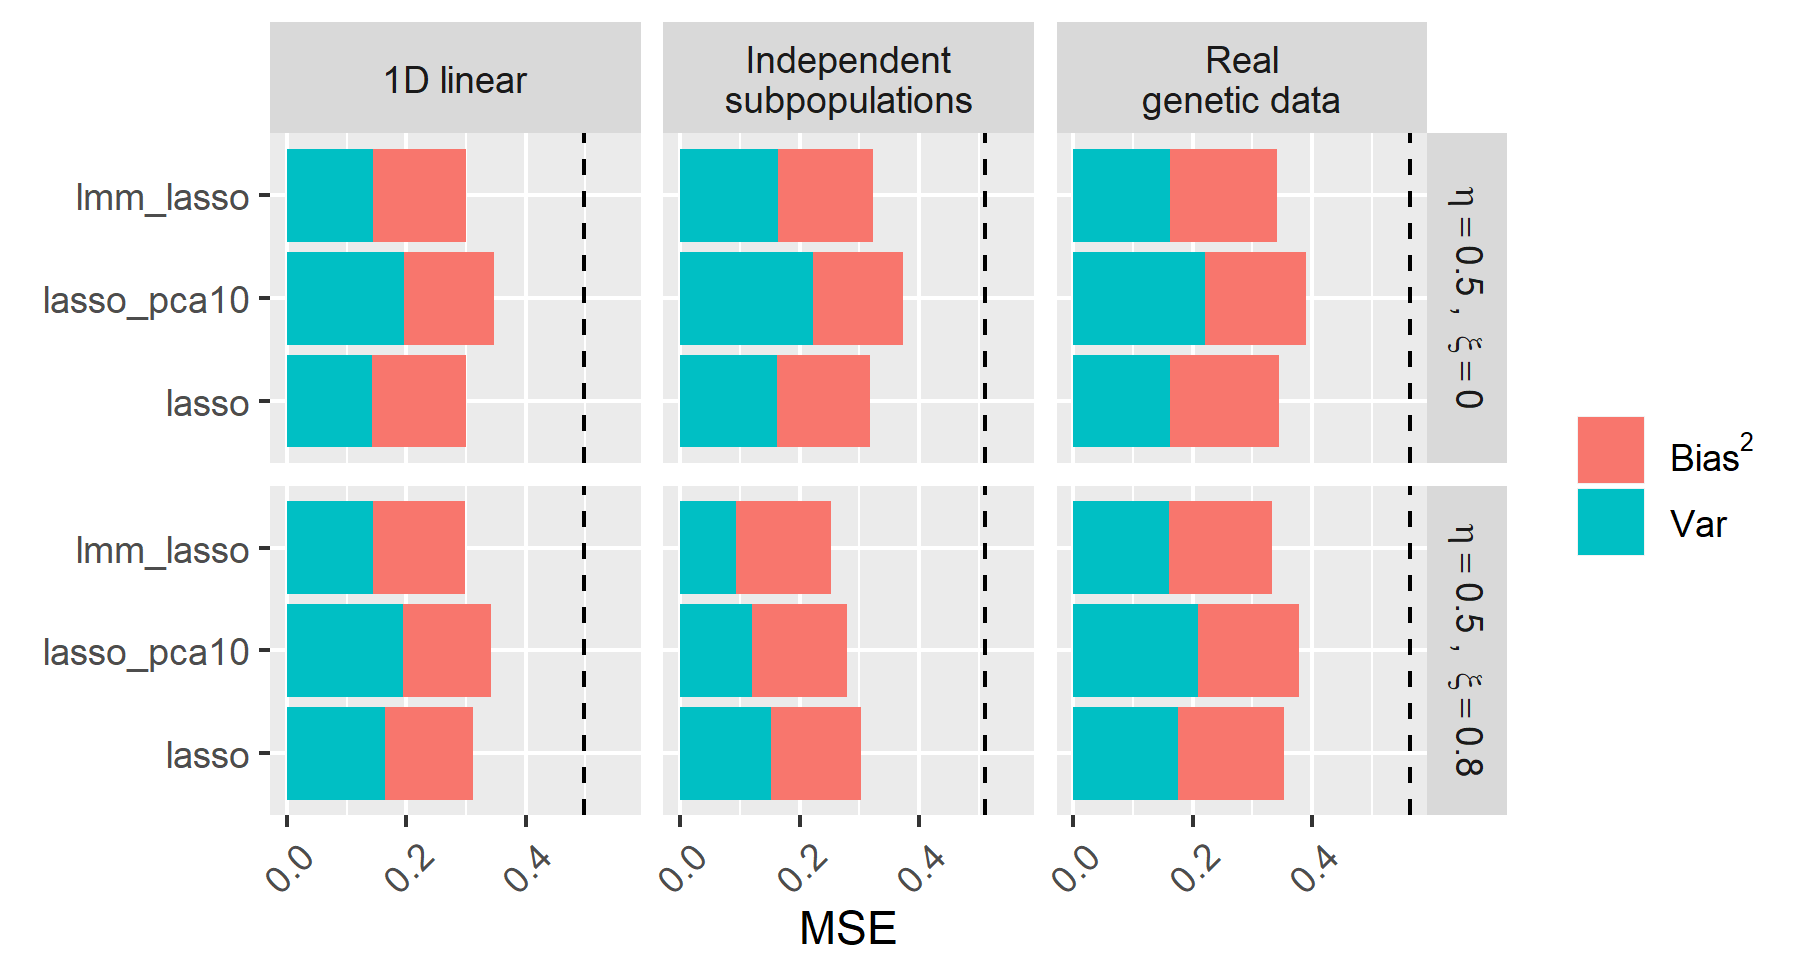
\includegraphics[scale = 0.7]{figures/fig1a.png}
    \caption{Low-dimensional setting ($n=200, p=100$)}
    \label{fig:ld}
\end{figure}

%------------------------------%
\subsection{PC-Lasso and LMM-Lasso outperform Lasso}
%------------------------------%
\begin{figure}[H]
    \centering
    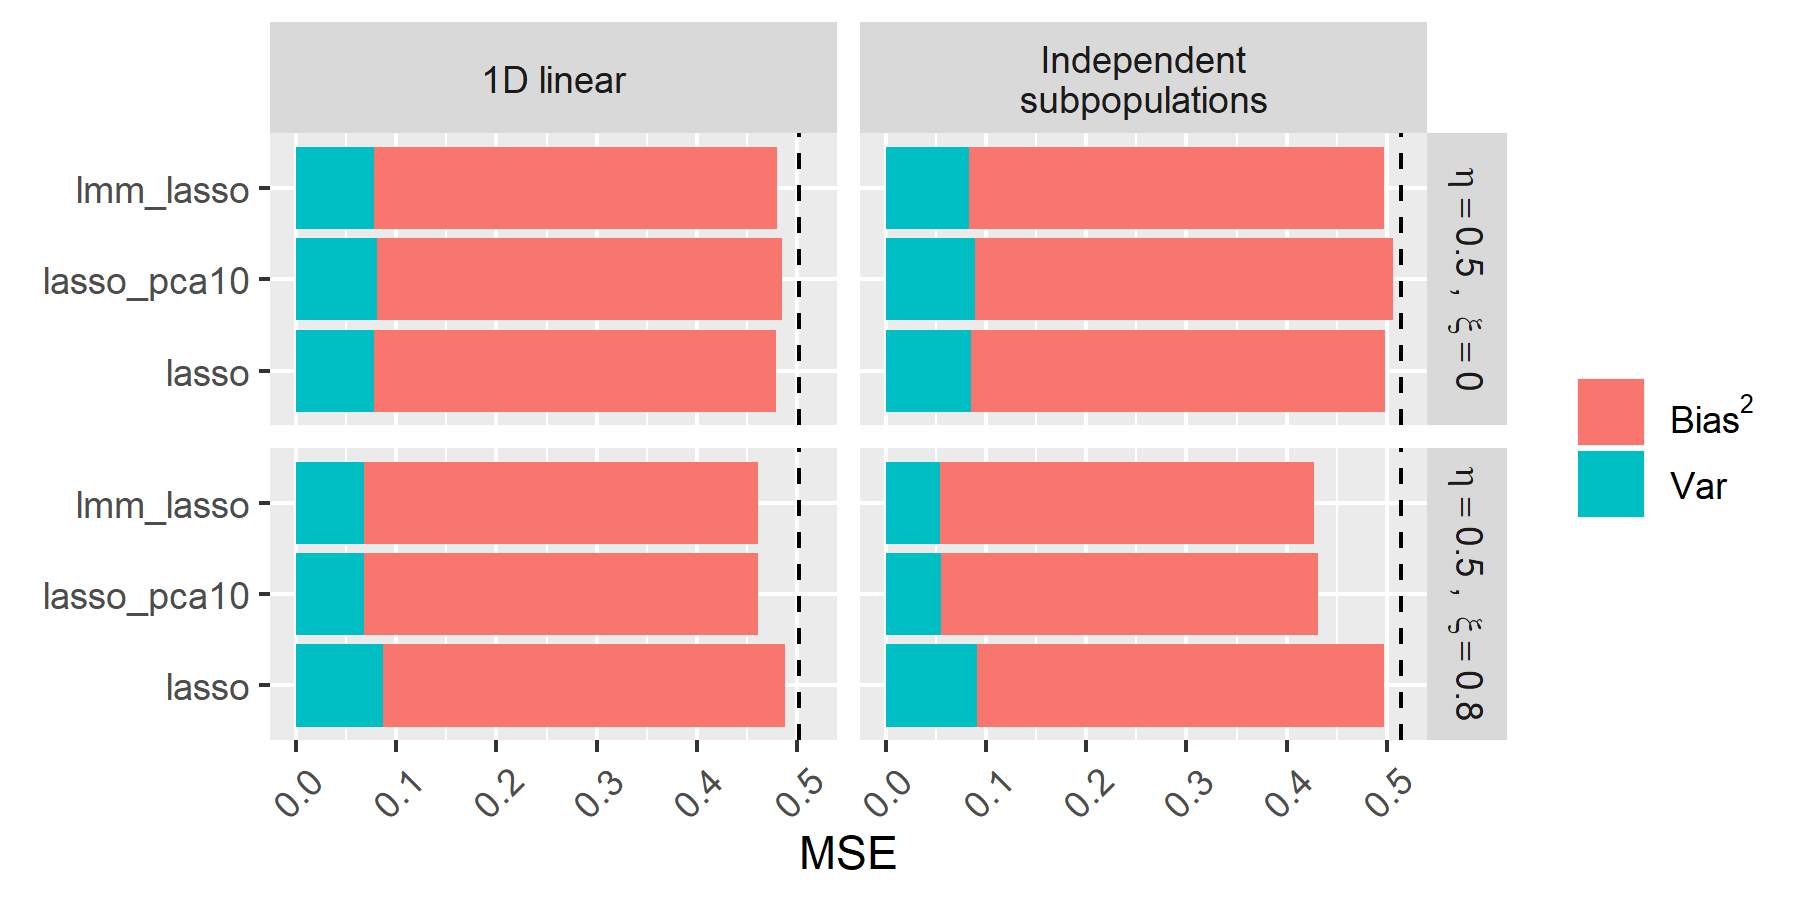
\includegraphics[scale = 0.7]{figures/fig1b.png}
    \caption{High dimensional setting ($n=200, p=1000$)}
    \label{fig:hd}
\end{figure}

\anna{add high-dimensional real data case using vanderwas?}

%------------------------------%
\subsection{Population structure}
%------------------------------%
\begin{figure}[H]
    \centering
    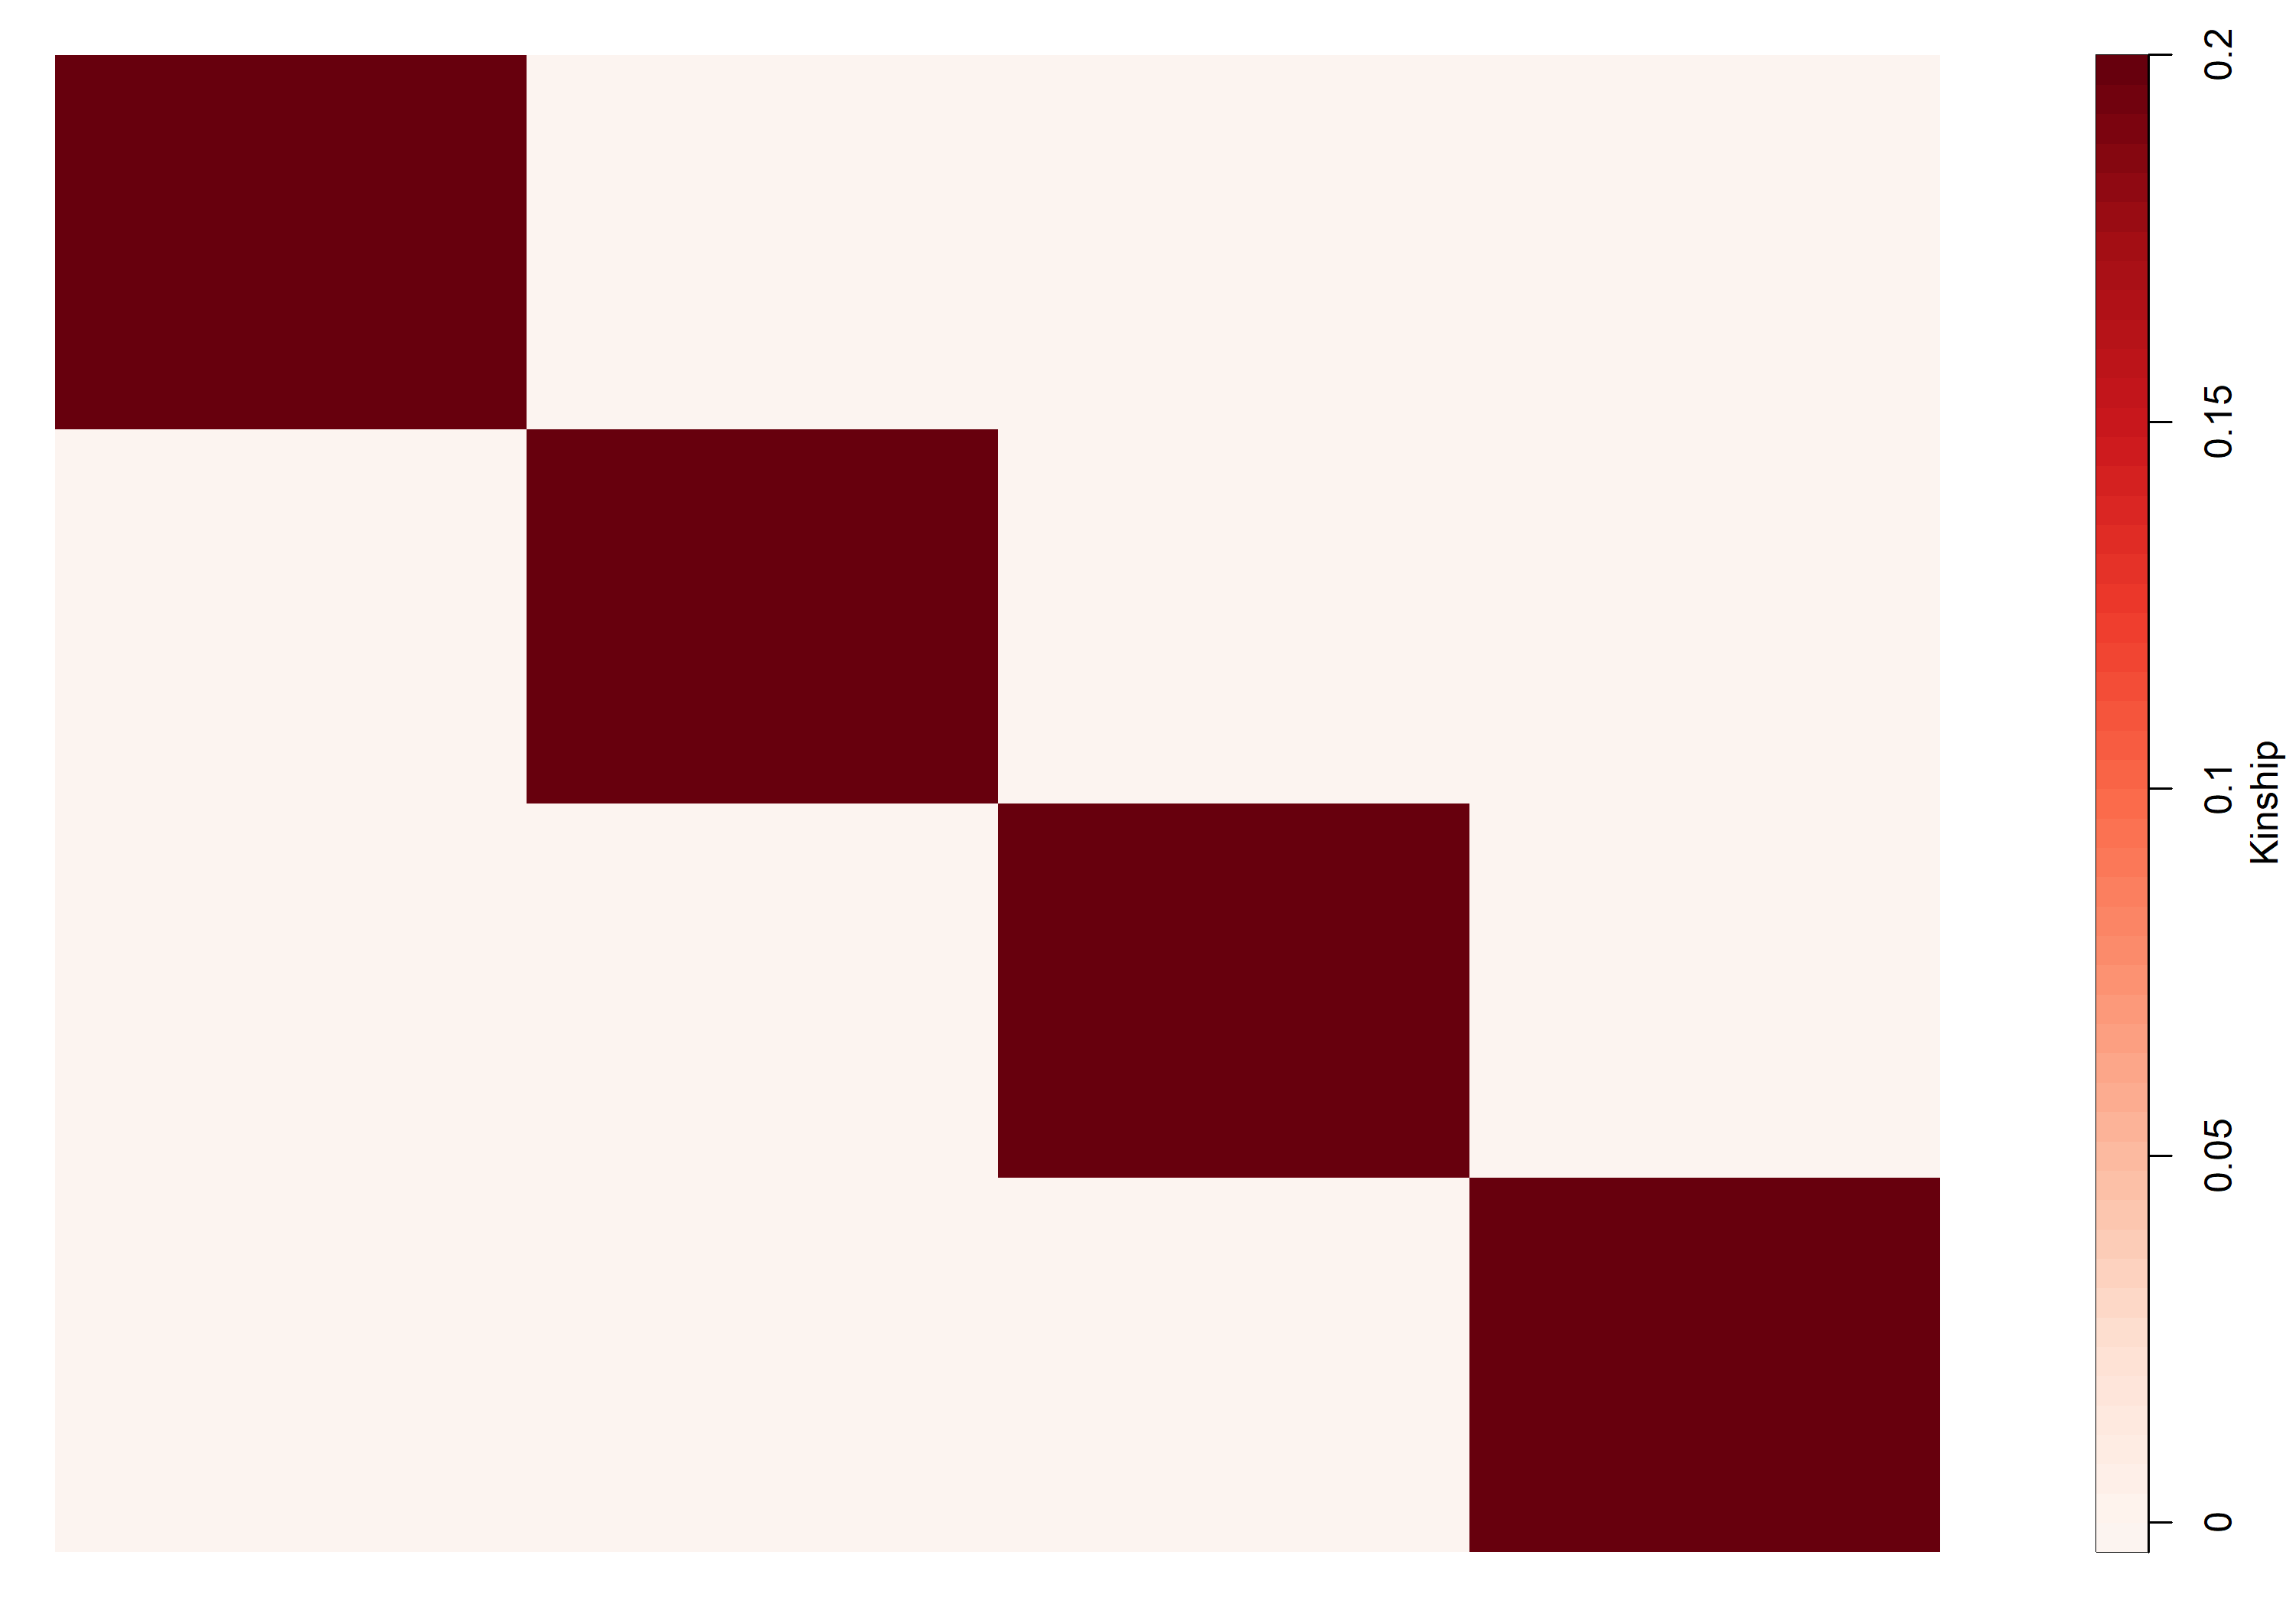
\includegraphics[scale = 0.7]{figures/kinship1}
    \caption{A few large subpopulations}
    \label{fig:big_blocks}
\end{figure}
\begin{figure}[H]
    \centering
    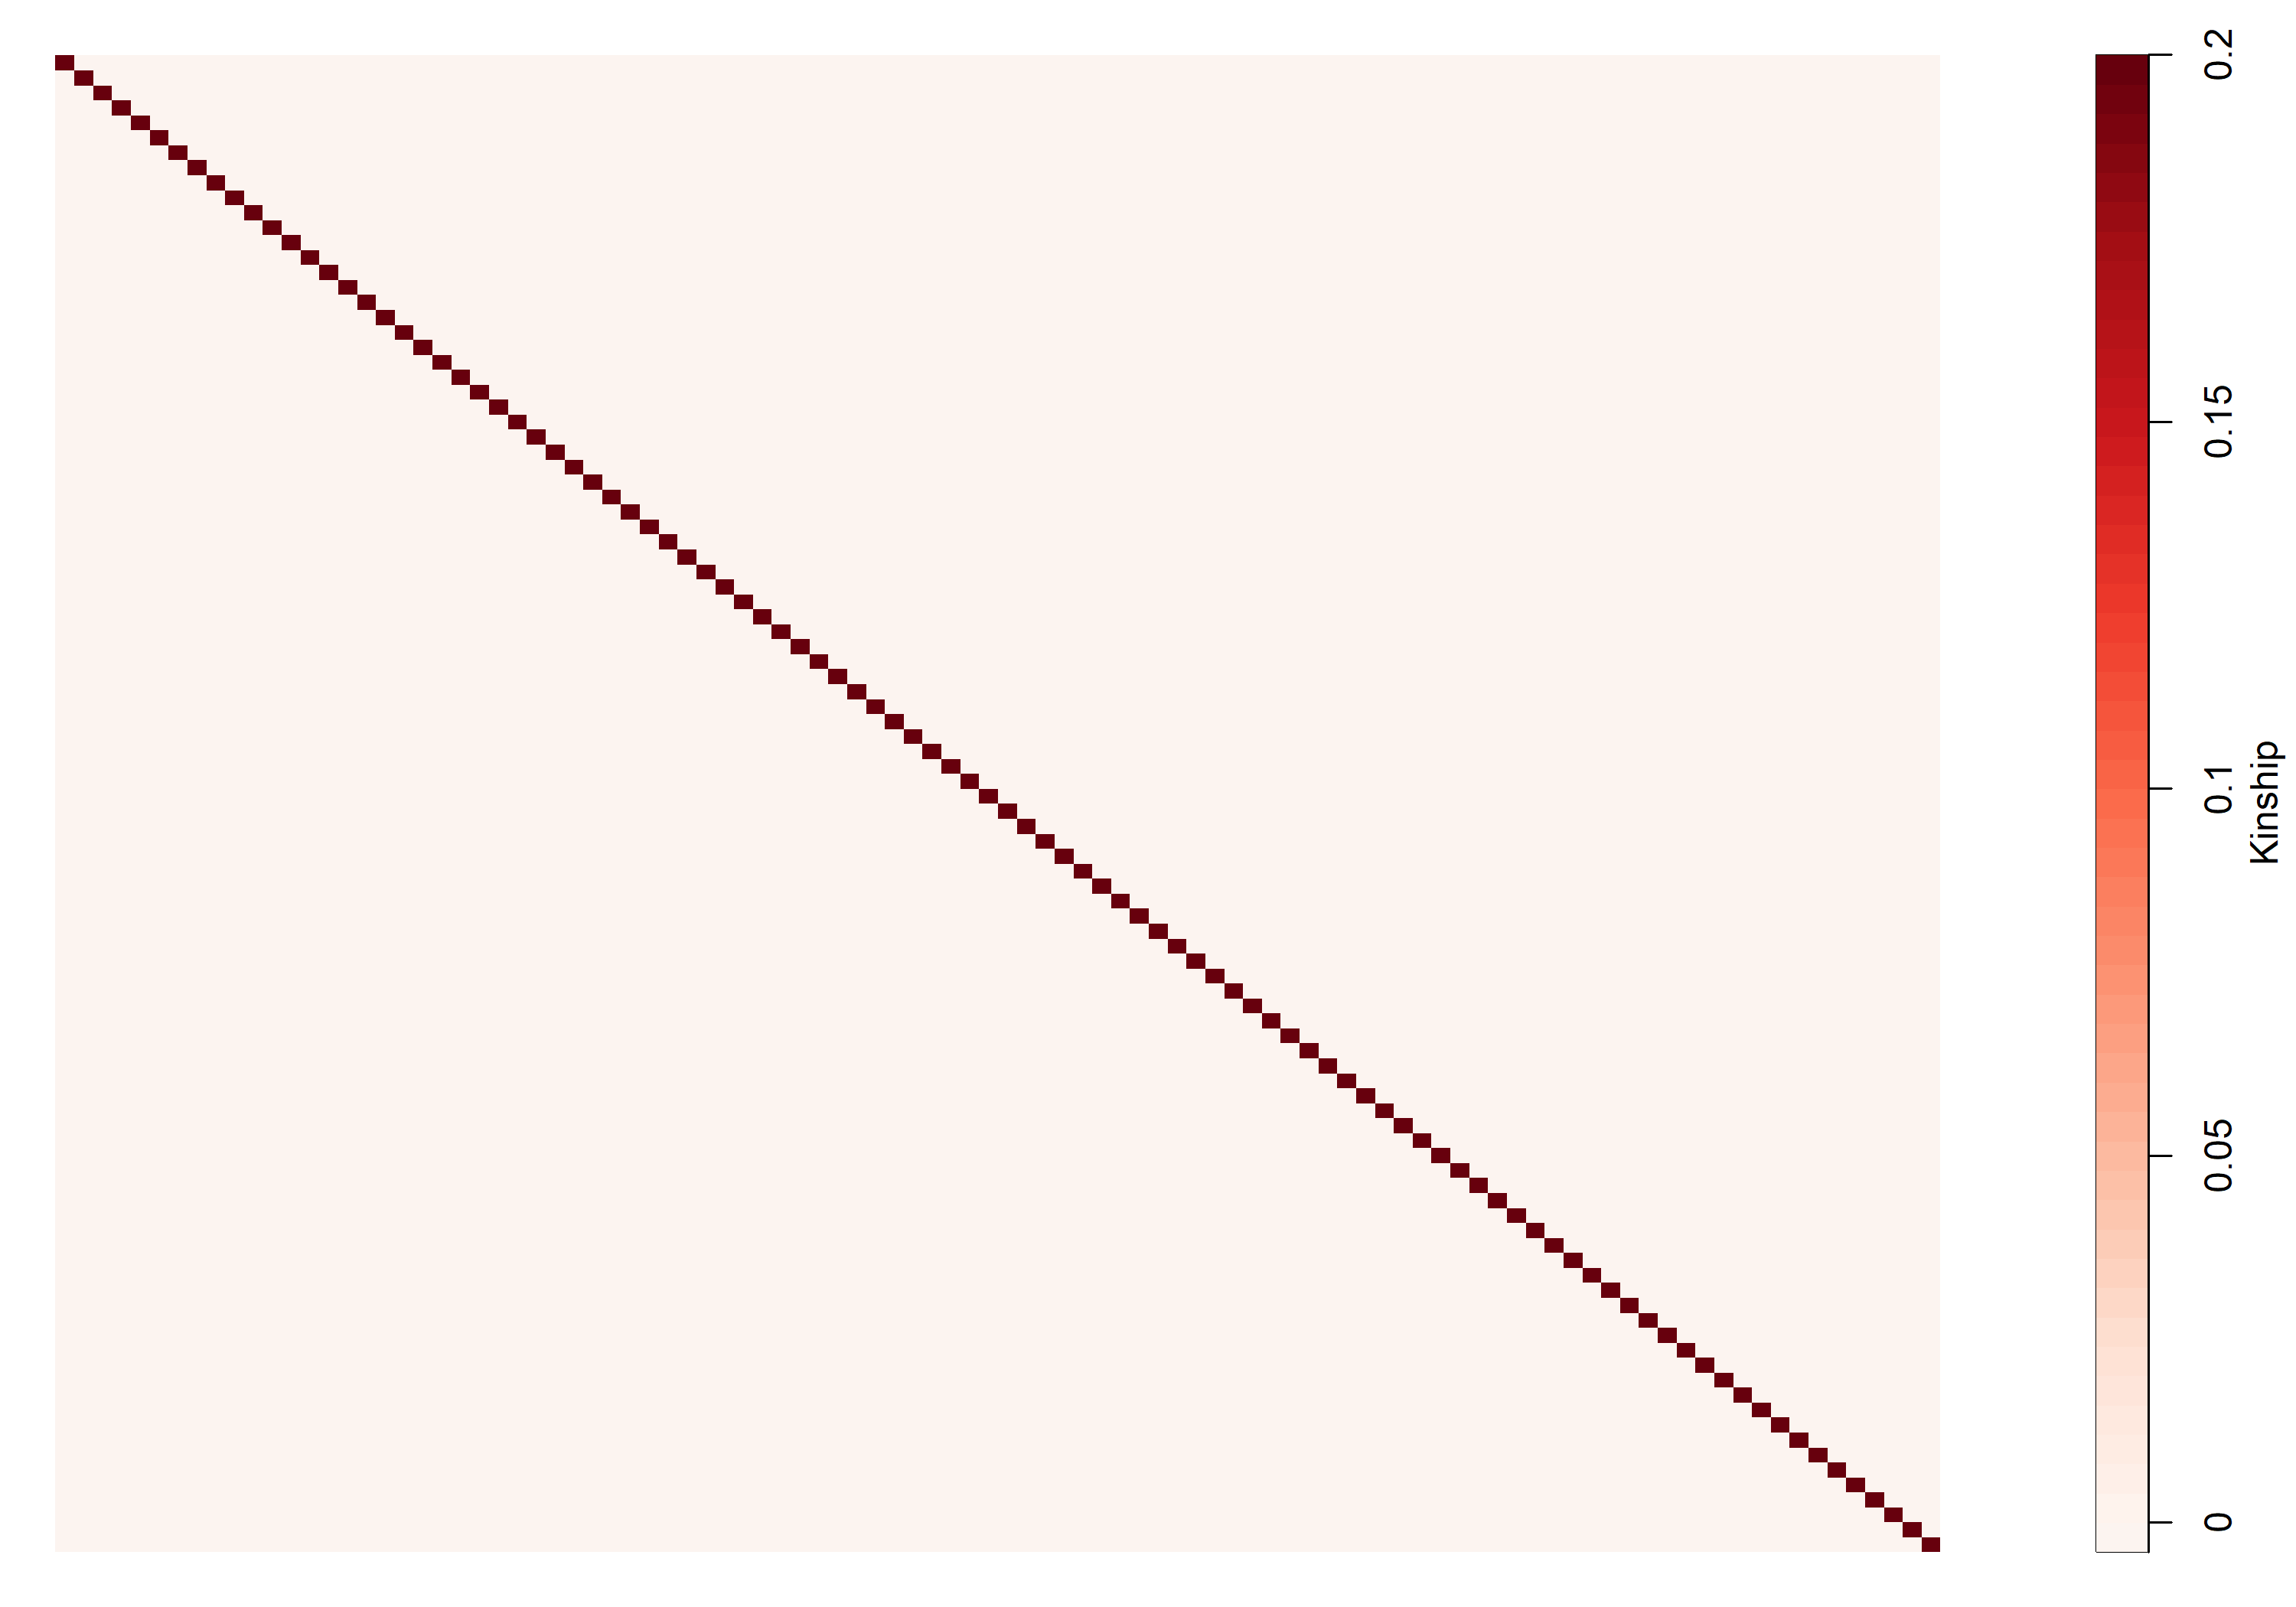
\includegraphics[scale = 0.7]{figures/kinship2}
    \caption{Many small subpopulations}
    \label{fig:small_blocks}
\end{figure}

%------------------------------%
\subsection{LMM-Lasso outperforms PC-Lasso when simulated subpopulations are small}
%------------------------------%
\begin{figure}[H]
    \centering
    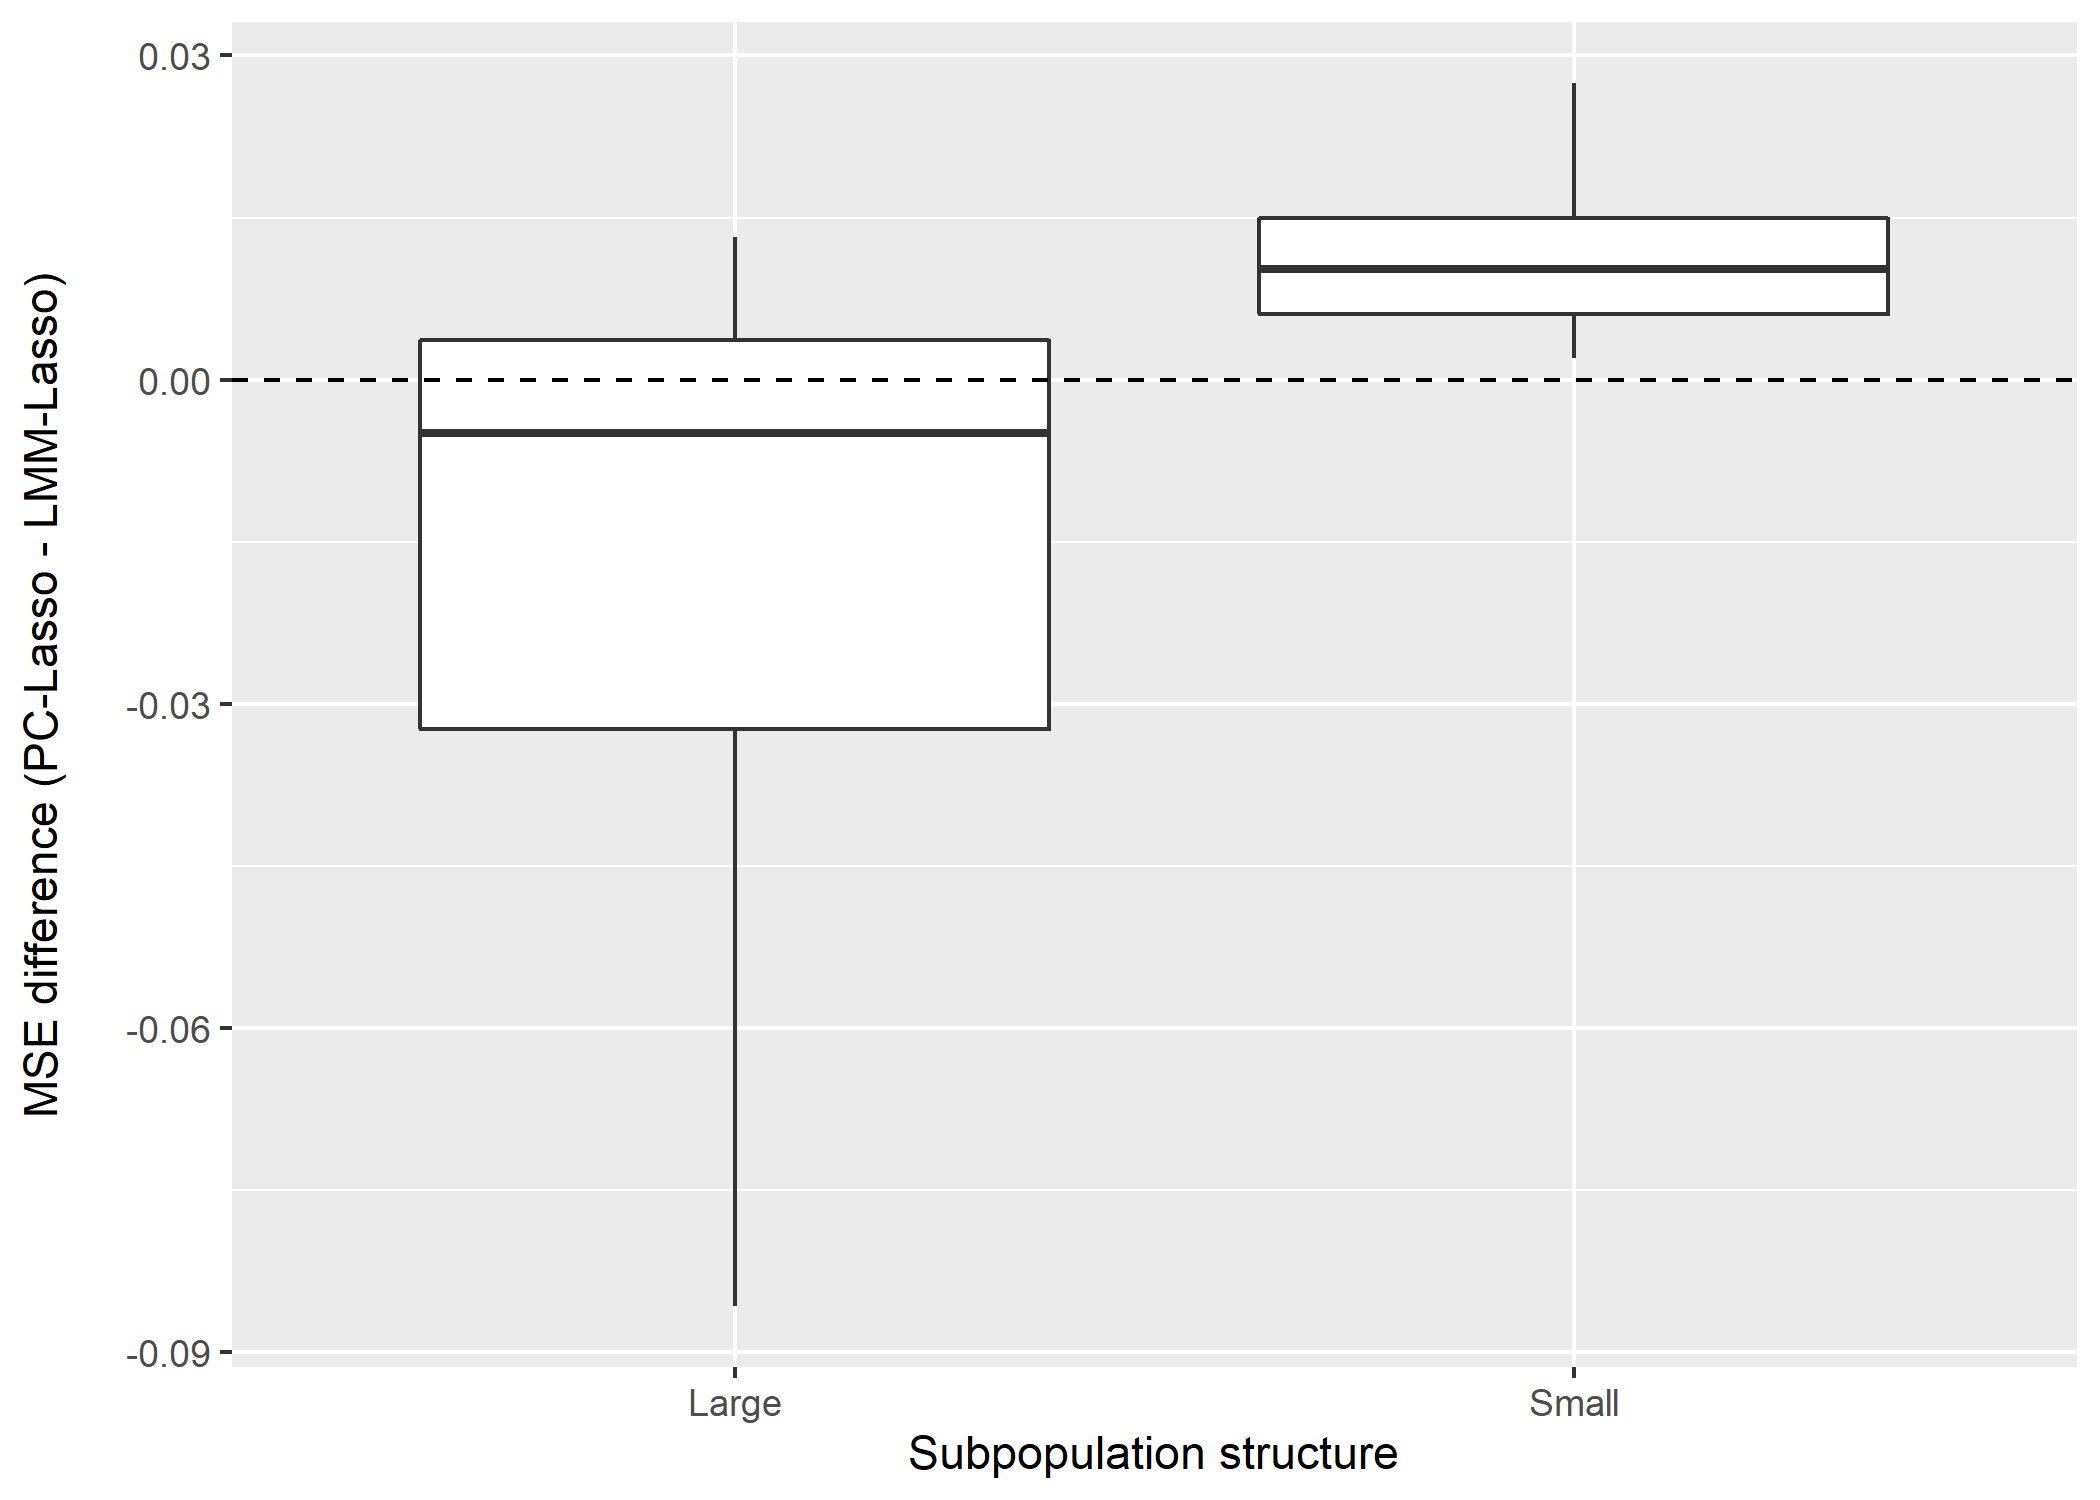
\includegraphics[scale = 0.7]{figures/fig2a}
    \caption{Relative performance of LMM-Lasso, PC-Lasso in terms of estimation accuracy.}
    \label{fig:big_vs_small}
\end{figure}

%------------------------------%
\subsection{$\gamma$ structure}
%------------------------------%
\begin{figure}[H]
    \centering
    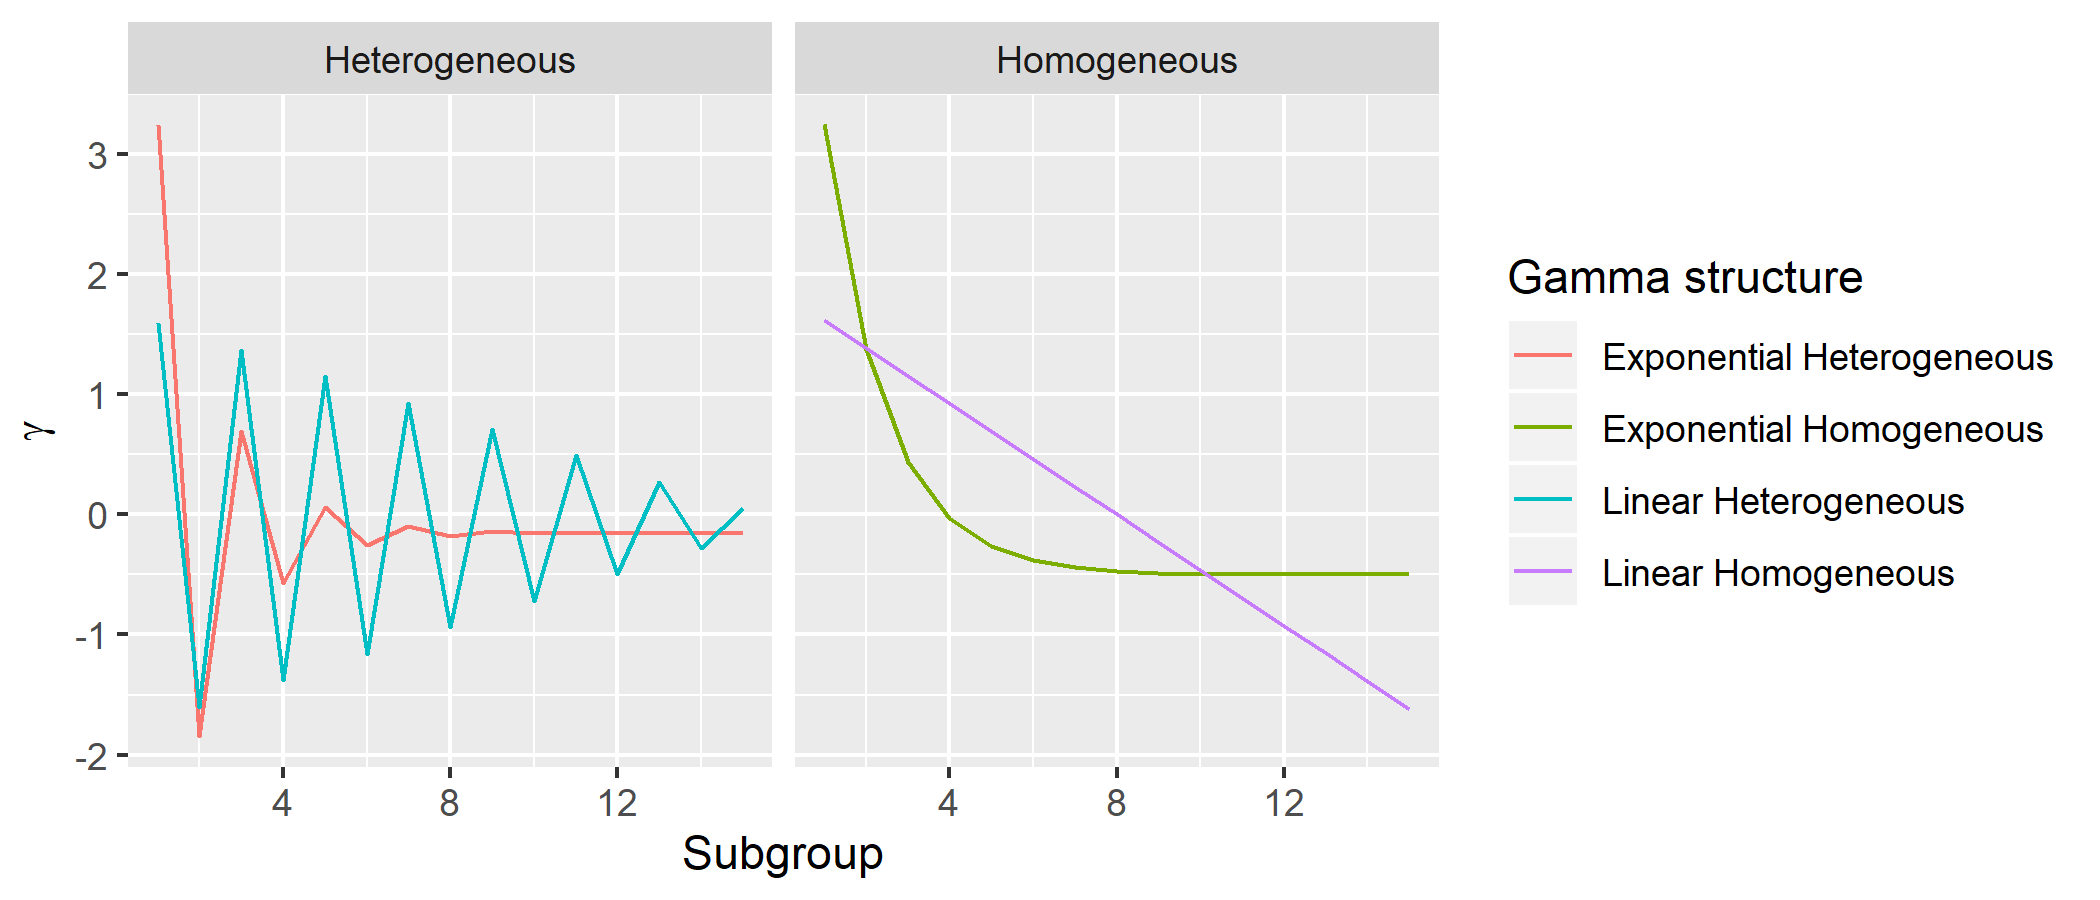
\includegraphics[scale = 0.7]{figures/gamma_structure.png}
    \caption{$\bgamma$ structures}
    \label{fig:gamma_structures}
\end{figure}


%------------------------------%
\subsection{LMM-Lasso outperforms PC-Lasso when $\gamma$ is heterogeneous}
%------------------------------%
\begin{figure}[H]
    \centering
    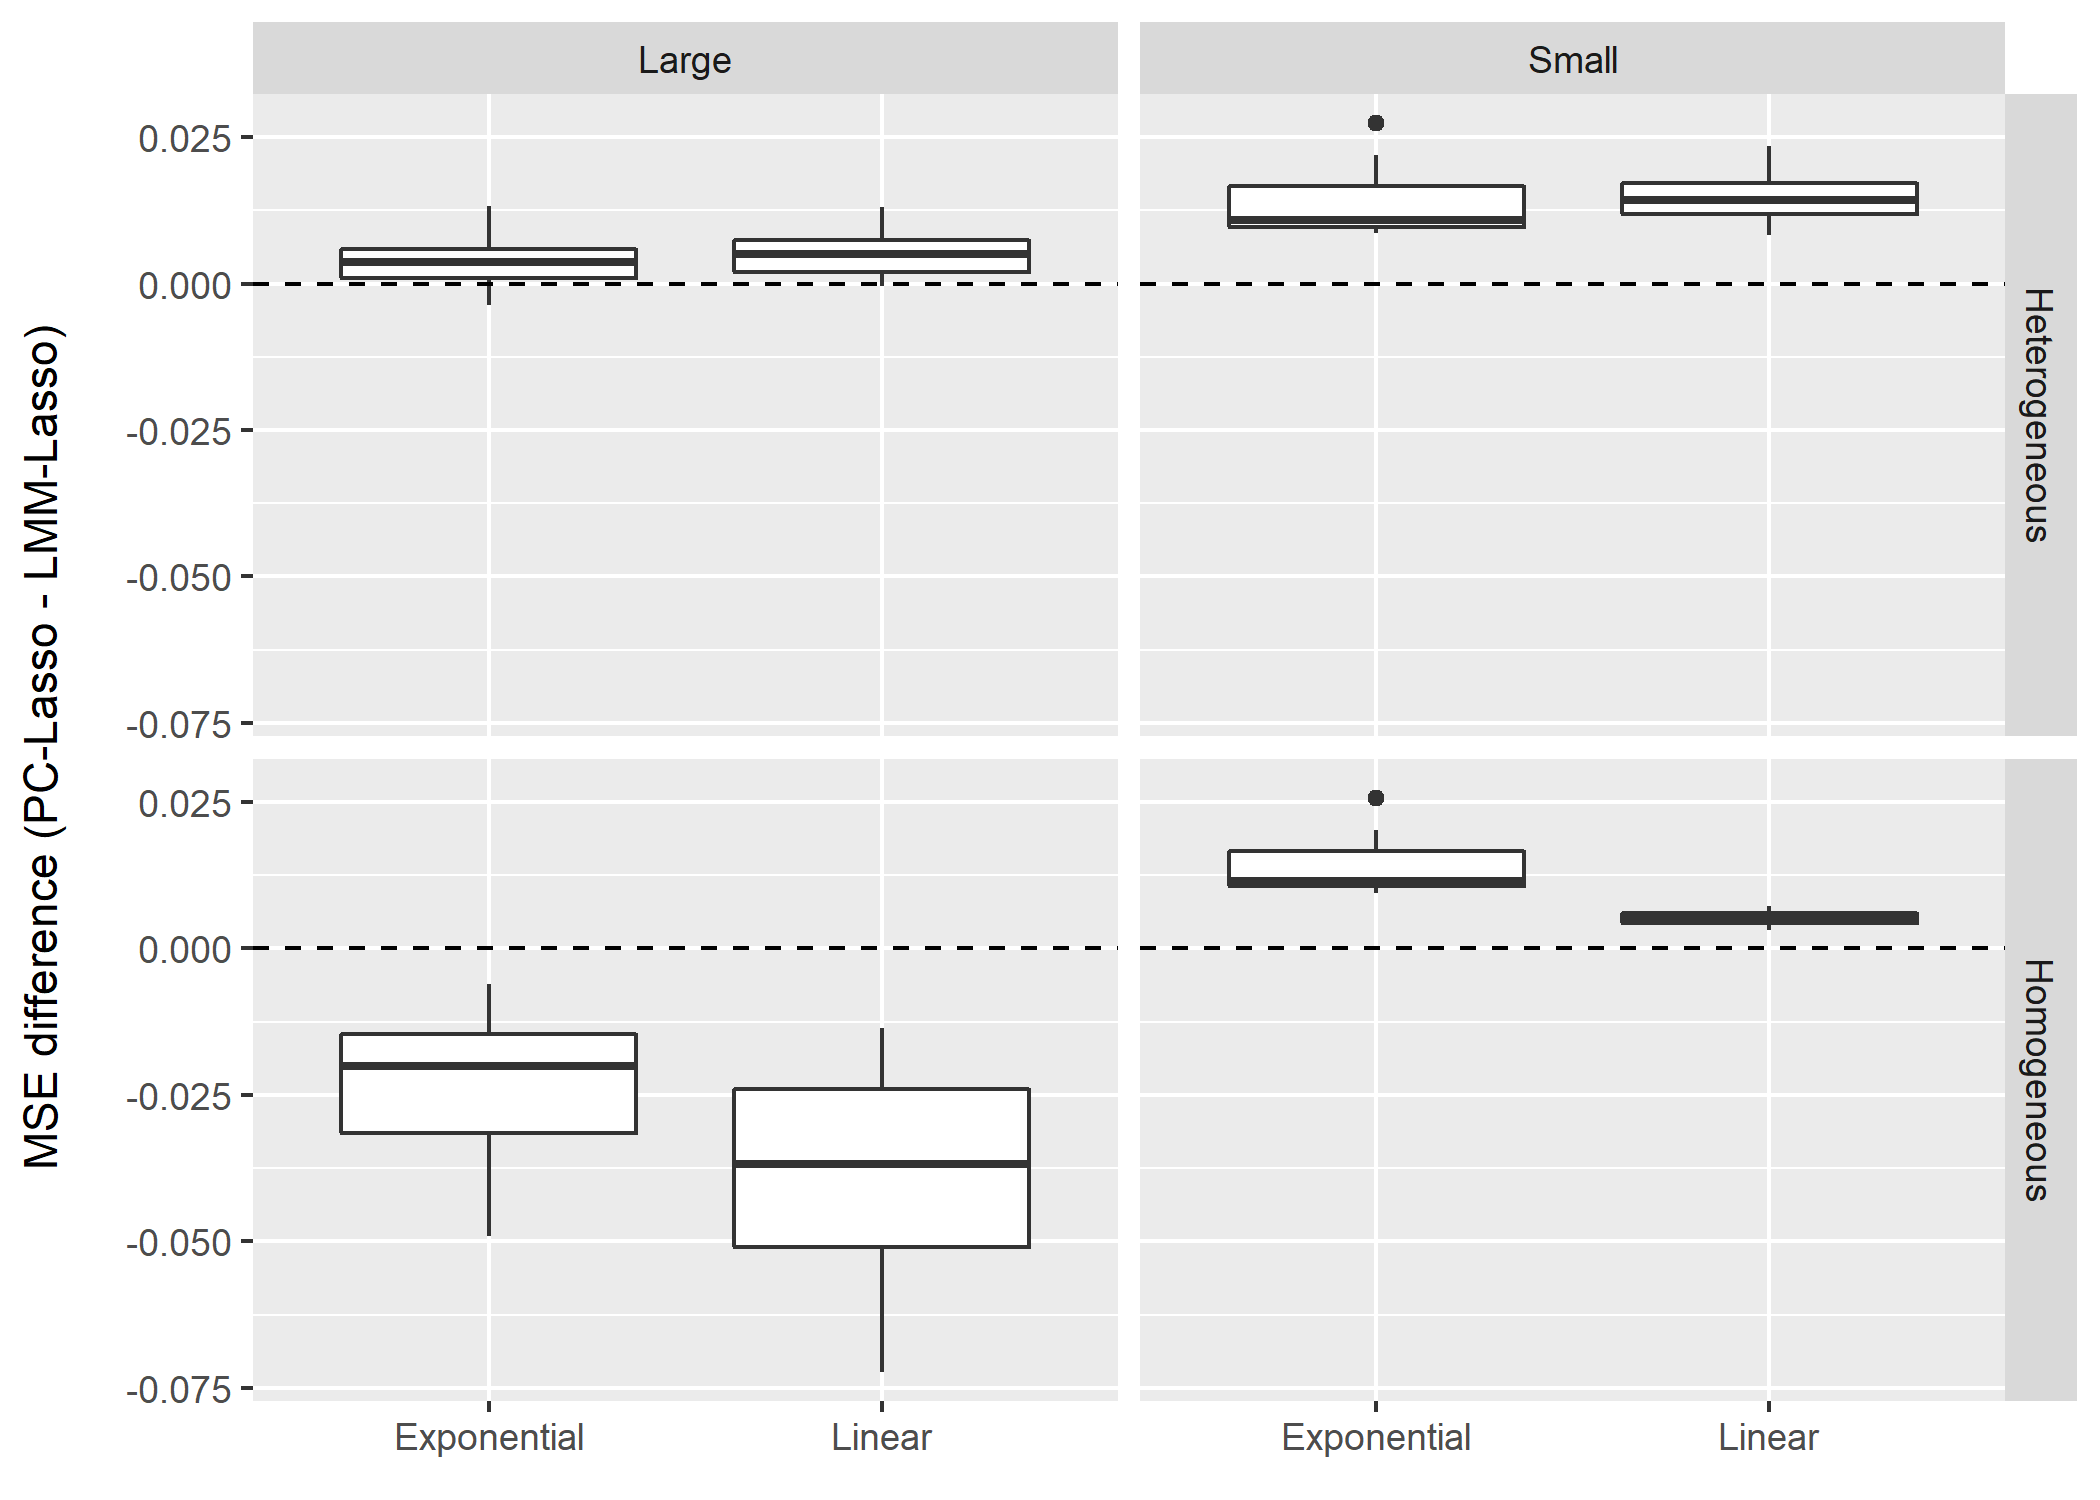
\includegraphics[scale = 0.9]{figures/fig2b.png}
    \caption{Relative performance of LMM-Lasso, PC-Lasso for different subpopulation and $\bgamma$ structures}
    \label{fig:my_label}
\end{figure}

%------------------------------%
\subsection{Re-estimation of $\eta$ may, in some cases, slightly improve our estimate of $\hat{\eta}$, but does not improve the estimation of $\beta$, and takes a long time}
Put this at the end of results
%------------------------------%

\anna{We have been unable to find a scenario where ggmix outperforms the LMM-Lasso method implemented by \cite{Rakitsch2012}. Ggmix performs poorly in a low-dimensional setting due to the ill-conditioning of the matrix K. Although it is primarily intended for use in high dimensional settings, where it performs on par with LMM-Lasso, this is also the scenario where it is ~100 times slower than LMM-Lasso. }\\

\anna{ggmix vs lmmlasso eta-hat plot} - I have this, make it pretty\\

\anna{ggmix vs lmmlasso MSE plot}- I have this, make it pretty\\

\anna{ggmix vs lmmlasso prc plot (?)}\\

\anna{ggmix vs. lmmlasso time plot}- I have this, make it pretty\\



%%%%%%%%%%%%%%%%%%%%%%%%%%%%%%%%
%------------------------------%
%%%%%%%%%%%%%%%%%%%%%%%%%%%%%%%%
\section{Discussion/conclusion}
%%%%%%%%%%%%%%%%%%%%%%%%%%%%%%%%
%------------------------------%
%%%%%%%%%%%%%%%%%%%%%%%%%%%%%%%%
\begin{itemize}
    \item LMM-Lasso outperforms PC-Lasso when (1) subpopulations are small and (2) when confounding effects are nonlinear and heterogeneous
    \item LMM-Lasso \cite{Rakitsch2012} and ggmix  \cite{bhatnagar2019simultaneous} perform similarly in many scenarios
    \item However, ggmix is time-consuming and may not be practical for more realistic genetic data sets
    \item Both PC-Lasso and LMM-Lasso methods suffer in estimation accuracy due to their bias from $\lambda$
    \item Bias-reduction techniques for penalized LMMs may be an attractive avenue for future work
\end{itemize}
